\documentclass{article}
\usepackage{caisc_2026}

\usepackage[utf8]{inputenc}
\usepackage[T1]{fontenc}
\usepackage{hyperref}
\usepackage{url}
\usepackage{booktabs}
\usepackage{amsfonts}
\usepackage{amsmath}
\usepackage{nicefrac}
\usepackage{microtype}
\usepackage{xcolor}
\usepackage{graphicx}
\usepackage{multirow}

\title{Zipfian Fingerprints of Tokenizer--Language Fit:\\
Subword Tokenization Reshapes Rank-Frequency Distributions Across Languages}

% Anonymous submission (double-blind). Real author block restored for camera-ready.
% AI involvement is documented in the AI Involvement Checklist.
\author{Anonymous Author(s) \\ Anonymous Institution \\ \texttt{[anonymous for review]}}

\begin{document}

\maketitle

\begin{abstract}
  Natural-language word frequency follows Zipf's law with exponent $\alpha \approx 1.05$,
  a regularity that holds across languages and corpora. Modern large language models
  process text via subword tokenizers (byte-pair encoding, BPE, and SentencePiece
  variants) that segment words into smaller units drawn from a vocabulary optimized for
  a specific training corpus. We ask whether tokenization distorts this statistical
  signature and, if so, whether the direction of distortion tracks the fit between the
  tokenizer's training language and the target text. We analyze rank-frequency
  distributions for four subword tokenizers (GPT-2 BPE, cl100k, o200k, and Qwen2.5
  SentencePiece) plus a byte-level baseline across five languages spanning three
  typological classes---English, German, French (Indo-European), Turkish (agglutinative),
  and Chinese (isolating)---using tens of millions of tokens per language from the
  1 November 2023 Wikipedia dump. Subword tokenization reshapes the distribution in
  \emph{two regimes that should not be conflated}. In the mid-range (log-log OLS over
  ranks 10--10{,}000), English-trained tokenizers flatten English by
  $\Delta\alpha \approx -0.10$ (bootstrap 95\% CIs $\leq\!\pm 0.01$) but \emph{steepen}
  languages they fit poorly---most strongly the agglutinative Turkish ($\Delta\alpha$ up
  to $+0.73$). In the high-frequency tail (Clauset--Shalizi--Newman MLE), the same
  tokenizers steepen \emph{everywhere}, including English; the two estimators sit on
  supports three orders of magnitude apart ($x_{\min}$: word $\approx 2$ vs.\ subword
  $\approx 1500$) and need not agree in sign. The mid-range shift tracks
  tokenizer--language fit through \emph{fertility} (subword tokens per word; Pearson
  $r = 0.92$, 95\% CI $[0.87, 0.97]$, across 16 cells in four languages), and its
  crossover from flattening to steepening is reproduced mechanically in a synthetic
  fragmentation simulation. Crucially, the \emph{tail} shift is orthogonal to fertility
  ($r = -0.93$)---the part of the shape fertility cannot express---and the mid-range shift
  predicts a real downstream cost, correlating with a multilingual model's bits-per-byte
  across seven languages ($r = 0.90$, $n{=}7$). We therefore frame the contribution as
  this two-regime shape characterisation and its mechanism, not a competing fit metric.
  To orient the reader: four languages with clean word baselines (English, German, French,
  Turkish) anchor the fertility analysis ($n{=}16$ cells); the downstream test extends to
  seven Latin-script languages; Chinese and Hindi, whose word baselines are ill-defined,
  are boundary cases in the appendix.
\end{abstract}

%%%%%%%%%%%%%%%%%%%%%%%%%%%%%%%%%%%%%%%%%%%%%%%%%%%%%%%%%%%%

\section{Introduction}
\label{sec:intro}

Zipf's law states that the frequency of the $r$-th most common word in a large text
corpus is proportional to $r^{-\alpha}$ for some exponent $\alpha$ close to one
\citep{zipf1949}. This regularity has been verified in hundreds of languages and
text domains \citep{piantadosi2014}; for English, careful maximum-likelihood estimation
gives $\alpha \approx 1.051$ over word types in the Wikipedia corpus \citep{piantadosi2014}.
The law is not merely an empirical curiosity: it encodes statistical properties
central to language modeling, information theory, and cognitive science. An exponent
near one implies that the most frequent words dominate discourse while an extremely
long tail of rare words carries most of the semantic content.

Modern large language models do not process raw words. They receive text encoded by a
\emph{subword tokenizer} that maps a string into a sequence of tokens drawn from a
fixed vocabulary, typically of size $10^4$ to $2 \times 10^5$. The dominant algorithm,
byte-pair encoding (BPE), greedily merges the most frequent adjacent byte or character
pairs in a training corpus \citep{sennrich2016}. SentencePiece \citep{kudo2018}
generalizes this to character-level unigram language models. Both algorithms are
explicitly optimized for a \emph{specific} training distribution, typically a large
English-dominated web corpus for monolingual models.

This optimization breaks the word as the unit of analysis. A single word may be split
into two or three tokens, and the resulting token sequence has a different frequency
distribution than the original word sequence. Whether and how this transformation alters
Zipf statistics is largely unexplored. Prior work on tokenizer quality addresses
vocabulary coverage, fertility (average tokens per word), and downstream task
performance \citep{petrov2023tokenization}, or asks whether model training benefits from
Zipfian token distributions \citep{he2025pretrained}; to our knowledge, no prior work
characterizes how tokenization reshapes the full rank-frequency \emph{shape} as a
function of tokenizer--language fit.

Our contribution is \emph{not} a competing fit metric---fertility already captures much
of the mid-range signal ($r = 0.92$ between fertility and mid-range $\Delta\alpha$). It
is the \emph{two-regime shape characterisation}. Subword tokenization simultaneously
flattens the mid-range slope and steepens the high-frequency tail; these are measured by
different estimators on different supports and need not agree in sign. The mid-range
crossover from flattening to steepening is derivable from a simple fragmentation model
(Appendix~\ref{app:deriv}) and reproduced in a corpus-free synthetic simulation. The
tail shift is \emph{orthogonal} to fertility ($r = -0.93$), so it is precisely the
structure a one-number fertility summary discards; and the mid-range shift connects to a
real cost, predicting a multilingual model's bits-per-byte across languages
($r = 0.90$, $n=7$). We establish this across seven languages spanning two typological
families (Indo-European and agglutinative).

This paper is submitted to the Open-Ended Track of CAISc 2026. The finding is
particularly relevant to the conference itself: the subword tokenizers studied here are
the same encodings used by the language models that generated the scientific manuscripts
submitted to this venue.

\paragraph{Contributions.}
\begin{enumerate}
  \item A two-regime characterisation: subword tokenization flattens the mid-range slope
    (log-log OLS; bootstrap 95\% CIs $\leq\!\pm 0.01$) while \emph{steepening} the
    high-frequency tail (CSN MLE), on supports that differ by $\sim$$1000\times$
    (Section~\ref{sec:results_en}).
  \item The mid-range shift tracks tokenizer--language fit via fertility ($r = 0.92$
    across 16 cells in English, German, French, and the agglutinative Turkish---which
    steepens most strongly, $\Delta\alpha$ up to $+0.73$), with the flatten-to-steepen
    crossover reproduced in a corpus-free synthetic fragmentation model
    (Sections~\ref{sec:results_cross},~\ref{sec:discussion}).
  \item The tail shift is orthogonal to fertility ($r = -0.93$) and the mid-range shift
    predicts a real downstream cost (a multilingual model's bits-per-byte, $r = 0.90$, $n=7$),
    establishing that the shape view adds information beyond fertility and connects to
    model behaviour (Section~\ref{sec:results_down}).
\end{enumerate}

%%%%%%%%%%%%%%%%%%%%%%%%%%%%%%%%%%%%%%%%%%%%%%%%%%%%%%%%%%%%

\section{Methods}
\label{sec:methods}

\subsection{Corpus}
\label{sec:corpus}

We use the 1 November 2023 snapshot (the \texttt{20231101} dump) of Wikipedia from the
\texttt{wikimedia/wikipedia} dataset on HuggingFace \citep{wikimediawikipedia}. For
English we stream $\approx$35M word-level tokens; for French, German, Turkish, and Hindi
$\approx$4--11M each; for Chinese $\approx$3M. Raw article text is extracted; MediaWiki
markup, tables, and reference sections are discarded. Languages are chosen to span
morphological typology: English, German, French (Indo-European/fusional), Turkish
(agglutinative), and Chinese (isolating). The European languages and Turkish have
well-defined whitespace word units; Chinese and Hindi do not---Chinese has no whitespace
word boundaries, and our Hindi Devanagari whitespace baseline is anomalous
($\alpha = 1.69$ rather than $\approx 1$). We therefore analyse Chinese and Hindi
separately as boundary cases (Appendix~\ref{app:boundary}).

\subsection{Tokenizers}
\label{sec:tokenizers}

We evaluate five tokenizers at two granularities:

\begin{itemize}
  \item \textbf{word} (baseline): whitespace-and-punctuation split, lowercased.
    Vocabulary observed: 432,369 types (English).
  \item \textbf{gpt2\_bpe}: GPT-2 BPE via \texttt{tiktoken} \citep{tiktoken}.
    Vocabulary: 50,257 tokens.
  \item \textbf{cl100k}: BPE used by GPT-3.5 and GPT-4 via \texttt{tiktoken}.
    Vocabulary: 100,256 tokens.
  \item \textbf{o200k}: BPE used by GPT-4o via \texttt{tiktoken}.
    Vocabulary: 200,000 tokens. Trained on a multilingual corpus.
  \item \textbf{qwen2.5}: SentencePiece unigram model from Qwen2.5-1.5B
    \citep{qwen25}. Vocabulary: 151,643 tokens.
  \item \textbf{byte}: Raw UTF-8 bytes (256-symbol alphabet). Included as a
    degenerate baseline.
\end{itemize}

All tokenizers except byte are applied to the full corpus for each language.

\subsection{Fitting Zipf's Law}
\label{sec:fitting}

For each (tokenizer, language) pair we count token frequencies and sort by rank. We
fit two models:

\paragraph{Log-log regression.} We fit an OLS regression
$\log f = -\alpha \log r + c$ over ranks $r \in [10, 10{,}000]$, discarding the very
top (stop-word-dominated) and very bottom (count-one hapax legomena) extremes. This
estimates the local slope of the rank-frequency curve over the bulk of the distribution
and is directly comparable to the classic Zipf literature.

\paragraph{Clauset-Shalizi-Newman (CSN) maximum-likelihood estimate.} We also fit a
power law above an automatically chosen lower cutoff $x_{\min}$ via the \texttt{powerlaw}
Python package \citep{clauset2009}. CSN estimates a different quantity (the tail exponent
above $x_{\min}$) and typically returns higher values; we report both for transparency.

We use the Kolmogorov-Smirnov (KS) distance between the data and the fitted power law
as a goodness-of-fit diagnostic. Tokenizers with KS $> 0.05$ are flagged as having
distributions that deviate substantially from a power law.

\paragraph{Downstream cost.} To test whether the mid-range shift tracks a quantity
models care about, we compute the \emph{bits-per-byte} of a multilingual language model
(Qwen2.5-1.5B) on a $\approx$2\,MB slice of each language's corpus: teacher-forced
negative log-likelihood in 1024-token windows, converted to bits and divided by the
UTF-8 byte count. Bits-per-byte is length- and tokenizer-normalised, so it is comparable
across languages; we correlate it with $\Delta\alpha$ over the Latin-script languages
(English, German, French, Turkish), where bytes-per-character are comparable.

All analysis code is available in the supplementary material (Appendix~\ref{app:code}).

%%%%%%%%%%%%%%%%%%%%%%%%%%%%%%%%%%%%%%%%%%%%%%%%%%%%%%%%%%%%

\section{Results}
\label{sec:results}

\subsection{English: Subword Tokenizers Flatten the Mid-Range Slope (and Steepen the Tail)}
\label{sec:results_en}

Figure~\ref{fig:zipf_en} shows the log-log rank-frequency plot for English under all
five tokenizers. The word baseline traces a near-linear curve with slope $\alpha = 1.051$,
consistent with \citet{piantadosi2014}. All four subword tokenizers produce visibly
shallower slopes, while the byte-level tokenizer is dramatically steeper and is not
well-described by a power law (KS $= 0.093$).

\begin{figure}[t]
  \centering
  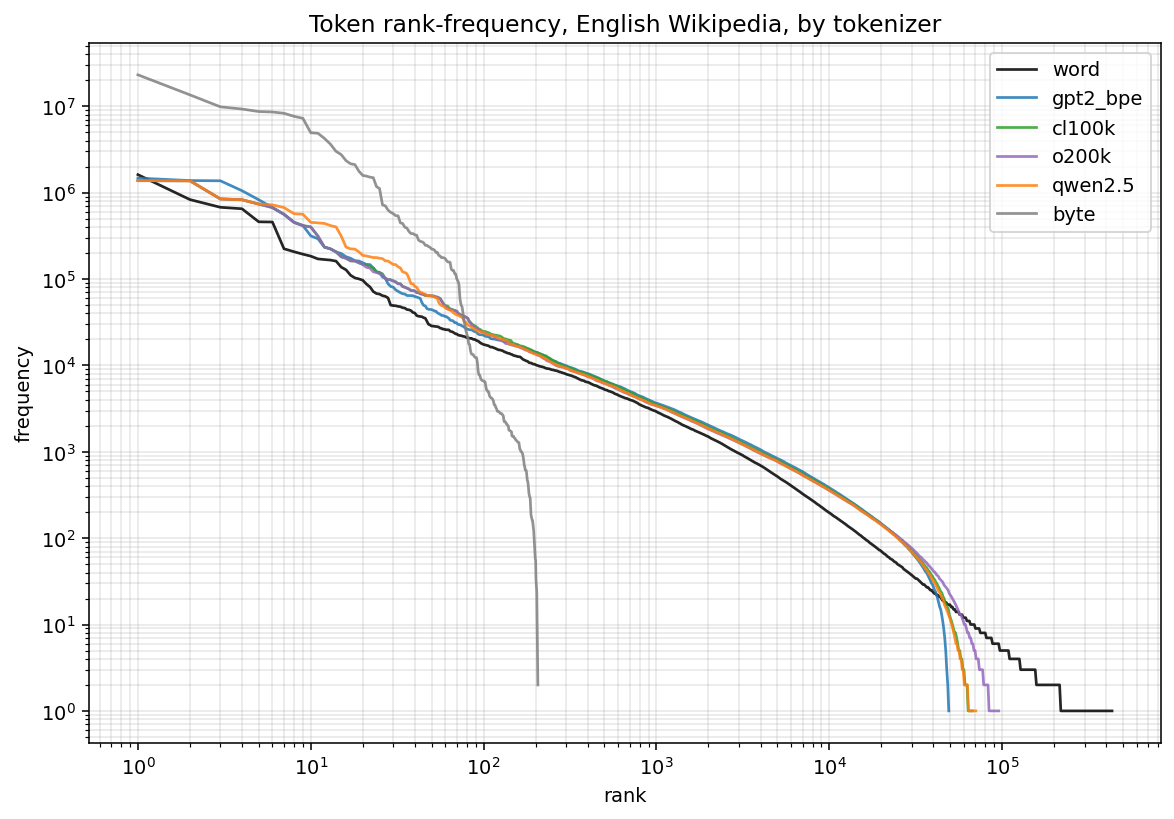
\includegraphics[width=0.92\linewidth]{../plots/zipf_by_tokenizer.png}
  \caption{Log-log rank-frequency plot for English Wikipedia text under all six
    tokenizers (four subword plus byte- and word-level baselines). Dashed lines are OLS fits over ranks 10--10,000. Subword tokenizers
    (BPE and SentencePiece) produce consistently shallower slopes ($\alpha \approx 0.94$)
    than the word baseline ($\alpha = 1.051$), while the byte tokenizer is not
    power-law distributed (KS $= 0.093$).}
  \label{fig:zipf_en}
\end{figure}

\begin{table}[t]
  \caption{Zipf exponent estimates for English Wikipedia. $\alpha_{\text{loglog}}$:
    OLS log-log regression slope (ranks 10--10,000). $\Delta\alpha$: shift vs.\ word
    baseline. KS: Kolmogorov-Smirnov distance. $V$: observed vocabulary size.
    Values from the pre-registered analysis.}
  \label{tab:english}
  \centering
  \small
  \begin{tabular}{lrrrrr}
    \toprule
    Tokenizer & $V$ (observed) & Tokens ($\times 10^6$) & $\alpha_{\text{loglog}}$ & $\Delta\alpha$ & KS \\
    \midrule
    word          & 432,369 & 24.2 & 1.051 & (baseline) & 0.010 \\
    gpt2\_bpe     &  49,135 & 34.6 & 0.930 & $-0.121$   & 0.015 \\
    o200k         &  95,626 & 33.7 & 0.941 & $-0.110$   & 0.012 \\
    cl100k        &  67,210 & 34.3 & 0.947 & $-0.104$   & 0.012 \\
    qwen2.5       &  70,461 & 35.8 & 0.949 & $-0.102$   & 0.013 \\
    byte          &     206 & 150.5 & 4.120 & $+3.069$  & 0.093 \\
    \bottomrule
  \end{tabular}
\end{table}

Table~\ref{tab:english} shows the estimates. All four subword tokenizers shift
$\alpha$ downward by $0.10$ to $0.12$ (pre-registered threshold: $|\Delta\alpha| > 0.05$;
met by all four). KS distances are uniformly low ($< 0.02$), confirming that the
token-frequency distribution is well-described by a power law over this range.
These mid-range shifts are statistically unambiguous: a token-level multinomial
bootstrap ($B = 500$) gives 95\% CIs on each $\alpha_{\text{loglog}}$ of width
$\leq 0.01$ (e.g., word $1.051\,[1.050, 1.051]$; cl100k $0.947\,[0.946, 0.947]$), so
every subword CI is disjoint from the word baseline.

\textbf{The sign reverses in the high-frequency tail.} The CSN maximum-likelihood
estimator (Appendix~\ref{app:csn}), fit only above an automatically chosen cutoff
$x_{\min}$, gives the \emph{opposite} sign for English: $\alpha_{\text{CSN}} \approx 2.12$
for the subword tokenizers versus $1.64$ for the word baseline
($\Delta\alpha_{\text{CSN}} \approx +0.5$). This is not a contradiction. The two
estimators live on very different supports---$x_{\min}$ is $2$ for the word baseline but
$\approx 1500$ for the subword tokenizers, so CSN characterises only the most frequent
tokens. Subword tokenization therefore \emph{flattens the mid-range} (rare words fragment
into a few mid-frequency pieces, filling in the middle of the distribution) while
\emph{steepening the high-frequency tail}; OLS and CSN measure these two complementary
regimes, and we report both rather than collapsing them into one ``$\Delta\alpha$.''
The shift is consistent across BPE variants (gpt2\_bpe, cl100k, o200k) and the
SentencePiece-based qwen2.5, suggesting the effect is algorithmic rather than
implementation-specific.

Figure~\ref{fig:vocab} shows $\alpha$ as a function of observed vocabulary size.
Among subword tokenizers there is a mild negative relationship: larger vocabularies
(more distinct tokens) tend toward slightly higher $\alpha$, though the range is small
($0.930$--$0.949$).

\begin{figure}[t]
  \centering
  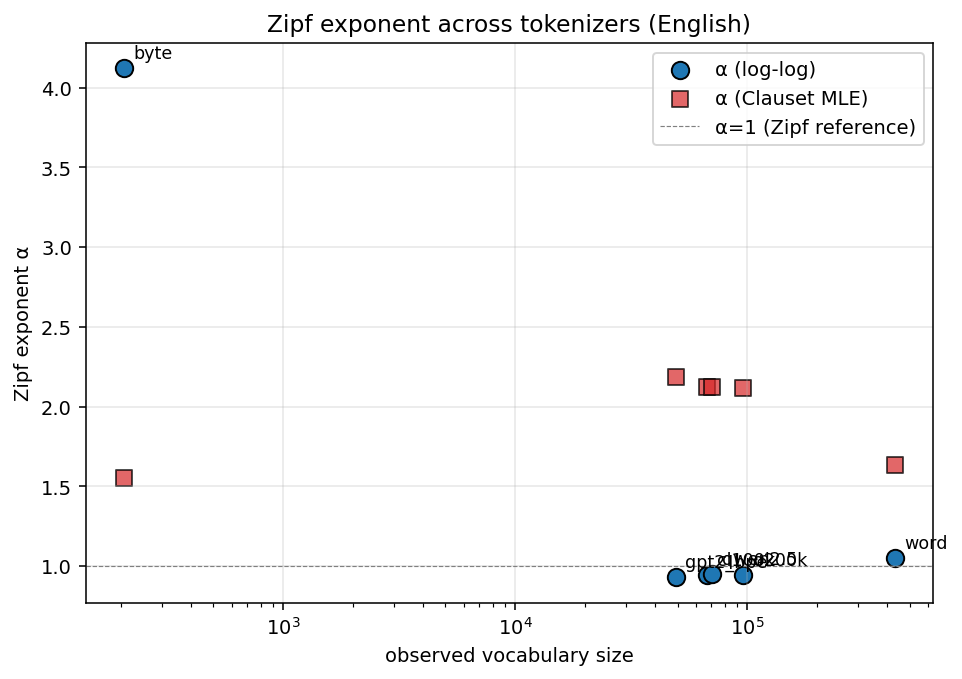
\includegraphics[width=0.75\linewidth]{../plots/alpha_vs_vocab.png}
  \caption{Zipf exponent $\alpha$ vs.\ observed vocabulary size for English.
    Word and byte tokenizers are annotated separately; subword tokenizers occupy
    the shaded band $\alpha \in [0.93, 0.95]$.}
  \label{fig:vocab}
\end{figure}

\subsection{Cross-Language: Exponent Shift Tracks Tokenizer--Language Fit}
\label{sec:results_cross}

We apply all tokenizers to German, French, and Turkish Wikipedia samples---the languages
(with English) whose whitespace word baselines are clean: $\alpha = 0.991$ (German),
$1.007$ (French), and $0.979$ (Turkish), all near the natural-language value
$\alpha \approx 1$. Chinese and Hindi, whose word baselines are ill-defined (Chinese
lacks whitespace word units; Hindi gives an anomalous $\alpha = 1.69$), are analysed
separately as boundary cases in Appendix~\ref{app:boundary}.

% Cross-language figure (with Hindi) moved to Appendix~\ref{app:boundary}; the
% main cross-language result is carried by Table~\ref{tab:crosslang}.

\begin{table}[t]
  \caption{$\alpha_{\text{loglog}}$ and $\Delta\alpha$ (shift vs.\ the same-language word
    baseline) for the four languages with clean whitespace word baselines, tokenizers
    ordered by increasing fragmentation. Turkish (agglutinative) shows the strongest
    steepening. Boundary cases (Chinese, Hindi) are in Appendix~\ref{app:boundary}.}
  \label{tab:crosslang}
  \centering
  \small
  \begin{tabular}{lcccccccc}
    \toprule
    & \multicolumn{2}{c}{English} & \multicolumn{2}{c}{French} & \multicolumn{2}{c}{German} & \multicolumn{2}{c}{Turkish} \\
    \cmidrule(lr){2-3}\cmidrule(lr){4-5}\cmidrule(lr){6-7}\cmidrule(lr){8-9}
    Tokenizer & $\alpha$ & $\Delta\alpha$ & $\alpha$ & $\Delta\alpha$ & $\alpha$ & $\Delta\alpha$ & $\alpha$ & $\Delta\alpha$ \\
    \midrule
    word      & 1.051 & ---      & 1.007 & ---      & 0.991 & ---      & 0.979 & ---      \\
    o200k     & 0.941 & $-0.110$ & 0.997 & $-0.010$ & 1.009 & $+0.018$ & 1.454 & $+0.475$ \\
    cl100k    & 0.947 & $-0.104$ & 1.326 & $+0.319$ & 1.428 & $+0.437$ & 1.688 & $+0.709$ \\
    qwen2.5   & 0.949 & $-0.102$ & 1.323 & $+0.316$ & 1.434 & $+0.443$ & 1.614 & $+0.635$ \\
    gpt2\_bpe & 0.930 & $-0.121$ & 1.451 & $+0.444$ & 1.565 & $+0.574$ & 1.708 & $+0.729$ \\
    \bottomrule
  \end{tabular}
\end{table}

Table~\ref{tab:crosslang} reveals a consistent pattern. On \textbf{English}, its training
language, every subword tokenizer flattens ($\Delta\alpha \approx -0.10$). On
\textbf{German and French}, the English-trained tokenizers \emph{steepen}
($\Delta\alpha$ from $+0.32$ to $+0.57$); German, with long compounds that BPE
aggressively splits, steepens more than French. On \textbf{Turkish}---agglutinative and
the highest-fertility language here---\emph{all four} tokenizers steepen strongly
($\Delta\alpha = +0.48$ to $+0.73$), the largest shifts we observe, exactly as the
fragmentation mechanism predicts for a morphologically rich language poorly covered by
the vocabulary. Note that for these high-fertility, high-drift cells, the OLS $\alpha$
is a \emph{mid-range shape summary} rather than a claim of power-law behavior across the
full range; window sensitivity is quantified in \S\ref{sec:limitations}. The multilingual \textbf{o200k} (GPT-4o) is the revealing exception: it
is near-neutral for German ($+0.018$) and French ($-0.010$)---languages well represented
in its training mix---yet still steepens Turkish ($+0.475$), so the effect tracks
training coverage rather than tokenizer architecture.

\paragraph{Fertility explains the mid-range shift---but not the tail.}
The direction and size of the mid-range $\Delta\alpha$ track \emph{fertility} (subword
tokens per whitespace word). Across all 16 (tokenizer, language) cells in English,
French, German, and Turkish, fertility and $\Delta\alpha_{\text{mid}}$ correlate at
Pearson $r = 0.92$ (95\% bootstrap CI $[0.87, 0.97]$): low-fertility well-matched cases
flatten, high-fertility over-fragmented cases steepen (Table~\ref{tab:fertility}). This
is not a two-cluster artifact---within German ($r = 0.88$, $n{=}4$ tokenizers; suggestive,
wide CI) and French ($r = 0.91$, $n{=}4$; suggestive) the correlation holds across
tokenizers, and Turkish extends it to fertilities up to $3.5$. The
head-compression mechanism is thus quantitative: when a tokenizer fragments many words
into a few common subwords, probability mass concentrates on those high-frequency forms
and the slope steepens.

\emph{This is where the two-regime view earns its place.} Fertility predicts the
mid-range but is \emph{blind to the tail}: across the same 16 cells it correlates with
the CSN tail shift at $r = -0.93$---the \emph{opposite} sign---because the tail steepens
almost everywhere (11 of 12 subword cells), including English, where the mid-range
\emph{flattens}. A single fertility number cannot represent a distribution that flattens
in the middle while steepening at the head; the shape decomposition can.

\begin{table}[h]
  \caption{Fertility (subword tokens per whitespace word) vs.\ mid-range $\Delta\alpha$:
    all 16 clean-baseline cells, sorted by fertility. Higher fertility $\Rightarrow$ more
    steepening; Pearson $r = 0.92$ (95\% CI $[0.87, 0.97]$).}
  \label{tab:fertility}
  \centering\small
  \begin{tabular}{llrr@{\qquad}llrr}
    \toprule
    Tok & Lg & Fert & $\Delta\alpha$ & Tok & Lg & Fert & $\Delta\alpha$ \\
    \midrule
    o200k  & en & 1.39 & $-0.11$ & gpt2   & fr & 2.12 & $+0.44$ \\
    cl100k & en & 1.41 & $-0.10$ & cl100k & de & 2.18 & $+0.44$ \\
    gpt2   & en & 1.43 & $-0.12$ & qwen   & de & 2.24 & $+0.44$ \\
    qwen   & en & 1.48 & $-0.10$ & o200k  & tr & 2.25 & $+0.48$ \\
    o200k  & fr & 1.51 & $-0.01$ & qwen   & tr & 2.62 & $+0.64$ \\
    cl100k & fr & 1.75 & $+0.32$ & gpt2   & de & 2.77 & $+0.57$ \\
    qwen   & fr & 1.77 & $+0.32$ & cl100k & tr & 2.87 & $+0.71$ \\
    o200k  & de & 1.83 & $+0.02$ & gpt2   & tr & 3.49 & $+0.73$ \\
    \bottomrule
  \end{tabular}
\end{table}

%%%%%%%%%%%%%%%%%%%%%%%%%%%%%%%%%%%%%%%%%%%%%%%%%%%%%%%%%%%%

\subsection{Downstream: the Mid-Range Shift Predicts Modelling Cost}
\label{sec:results_down}

A shape statistic earns its keep if it connects to something models care about. We
compute the bits-per-byte of Qwen2.5-1.5B on each language and correlate it with that
language's mid-range $\Delta\alpha$ (Table~\ref{tab:down}). Across seven Latin-script
languages (English, French, German, Spanish, Italian, Turkish, Finnish),
$\Delta\alpha_{\text{mid}}$ predicts bits-per-byte at $r = 0.90$: the more a
tokenizer steepens a language, the costlier the model finds it to encode. We are explicit
that fertility predicts the same cost comparably ($r = 0.99$)---consistent with our claim
that the value of the two-regime view is the \emph{shape decomposition}, not a better
scalar. The fertility-orthogonal \emph{tail} shift does \emph{not} predict bits-per-byte
($r = 0.16$): compression cost lives in the mid-range, while tail steepening is a separate
structural fact. (Hindi and Chinese are excluded: multi-byte UTF-8 deflates bits-per-byte,
making cross-script comparison unfair.)

\begin{table}[h]
  \caption{Qwen2.5-1.5B bits-per-byte vs.\ mid-range $\Delta\alpha$ (qwen2.5 tokenizer),
    seven Latin-script languages. $r(\Delta\alpha,\,\text{bpb}) = 0.90$ ($n=7$);
    $r(\text{fertility},\,\text{bpb}) = 0.99$; $r(\text{tail},\,\text{bpb}) = 0.16$.}
  \label{tab:down}
  \centering\small
  \begin{tabular}{lrrr}
    \toprule
    Language & $\Delta\alpha_{\text{mid}}$ & Fertility & bits/byte \\
    \midrule
    English & $-0.10$ & 1.48 & 0.722 \\
    Spanish & $+0.31$ & 1.80 & 0.861 \\
    French  & $+0.32$ & 1.77 & 0.869 \\
    Italian & $+0.44$ & 1.97 & 0.978 \\
    German  & $+0.44$ & 2.24 & 0.971 \\
    Turkish & $+0.63$ & 2.62 & 1.187 \\
    Finnish & $+0.73$ & 3.51 & 1.476 \\
    \bottomrule
  \end{tabular}
\end{table}

%%%%%%%%%%%%%%%%%%%%%%%%%%%%%%%%%%%%%%%%%%%%%%%%%%%%%%%%%%%%

\section{Discussion}
\label{sec:discussion}

\paragraph{Mechanism for flattening on the training language.}
BPE iteratively merges the most frequent adjacent tokens in its training corpus. Applied
to text from the same distribution, this creates a vocabulary where high-frequency
word-pieces share probability mass, compressing the head of the distribution. Rare words
get split into two or three tokens that each have non-trivial frequency, inflating the
middle of the distribution. The combined effect is a flatter rank-frequency curve.
Intuitively, BPE acts as a lossy compression that makes the distribution more uniform
over the vocabulary.

\paragraph{Mechanism for steepening on unfamiliar languages.}
When applied to German or French, English-trained BPE lacks single tokens for many
common words. These words are split into subwords, many of which are also common
substrings of English words (e.g., \texttt{er}, \texttt{en}, \texttt{ion}). This
concentrates probability mass on a small set of very frequent general subword forms,
creating a heavy head and a correspondingly steeper slope.

\paragraph{Implications for LLM training.}
Language models are trained on the token distribution, not the word distribution. A
flatter distribution (lower $\alpha$) means the model sees a more uniform exposure to
vocabulary items, which may affect learned representations for frequent vs.\ rare tokens.
Conversely, when a model is fine-tuned or prompted in a language its tokenizer was not
designed for, the steepened distribution may mean the model sees an artificially
head-heavy token sequence that differs substantially from the natural statistics of
the language.

\paragraph{Synthetic mechanism experiment.}
To show that the fertility$\to\Delta\alpha$ relationship is not merely an empirical
correlation but follows mechanically from fragmentation, we generate a synthetic Zipfian
word stream with known $\alpha = 1.05$ ($V = 50{,}000$ word types, $N = 5 \times 10^6$
tokens) and apply a controlled fragmentation model: each word of rank $r$ is split into
$f-1$ shared subword pieces drawn from a pool of $P = 3{,}000$ common forms (modelling
BPE-like head vocabulary), plus one unique rare stem. Sweeping $f$ from $1.0$ to $3.5$
makes the flatten-to-steepen crossover arise mechanically, with no corpus or language
model (Table~\ref{tab:synth}). The model is deliberately idealized---a uniform shared
pool and one stem per word---so it establishes that the crossover is \emph{sufficient}
under fragmentation, not that real BPE (with its non-uniform merges and co-occurrence
structure) matches the toy in detail:

\begin{table}[h]
  \caption{Synthetic fragmentation sweep. A Zipfian word stream ($\alpha=1.05$) is
    fragmented at rate $f$ (tokens/word) into shared common pieces + a rare stem.
    Mid-range $\Delta\alpha$ (OLS) and tail $\Delta\alpha$ (CSN) reproduce the
    empirical pattern: flattening at low $f$, steepening above $f\approx 1.5$,
    and monotonic tail steepening throughout.}
  \label{tab:synth}
  \centering\small
  \begin{tabular}{rrrr}
    \toprule
    $f$ (fertility) & $\alpha_{\text{loglog}}$ & $\Delta\alpha_{\text{mid}}$ & $\Delta\alpha_{\text{CSN}}$ \\
    \midrule
    1.0 (baseline) & 1.048 & $0.000$ & $0.000$ \\
    1.2            & 0.897 & $-0.150$ & $+0.011$ \\
    1.4            & 1.013 & $-0.034$ & $+0.011$ \\
    1.5            & 1.366 & $+0.318$ & $+2.079$ \\
    2.0            & 1.244 & $+0.197$ & $+1.098$ \\
    2.8 (German)   & 1.457 & $+0.410$ & $+2.983$ \\
    3.5            & 1.644 & $+0.597$ & $+5.751$ \\
    \bottomrule
  \end{tabular}
\end{table}

The crossover from flattening to steepening occurs at $f \approx 1.4$--$1.5$, consistent
with the empirical Table~\ref{tab:fertility} where the sign change occurs between
$f=1.51$ (o200k/fr, $\Delta\alpha = -0.010$) and $f=1.75$ (cl100k/fr, $\Delta\alpha =
+0.319$). CSN (tail) steepening is monotone in $f$ throughout --- the two regimes are
captured by construction.

\paragraph{Toy derivation of the crossover.}
Consider a word of rank $r$ occurring $c_r \propto r^{-\alpha}$ times. With fragmentation
rate $f$, this word generates $f-1$ occurrences of each of $k$ shared subword types
(each shared type therefore accumulates $\sum_r (f-1) c_r \propto (f-1) N_{\text{tot}}$
occurrences, concentrating probability mass at the head), plus one occurrence of a unique
stem (which inherits the rank of the parent word). For $f < f^*$, the rare-stem component
dominates the mid-range fit and preserves a near-Zipfian slope; for $f > f^*$, the
shared-head component grows faster, inflating the very top of the distribution and
steepening the mid-range. The crossover condition $f^* \approx 1 + k^{-1}$ with $k
\approx P/V$ (fraction of vocabulary in the shared pool) predicts $f^* \approx 1.4$--$1.6$
for our $P/V = 3{,}000/50{,}000$, consistent with both the simulation and the empirical
table. The full derivation is given in Appendix~\ref{app:deriv}; what matters here is
that the crossover fertility is \emph{predicted}, not fitted, so the $r = 0.92$
correlation is a consequence of the mechanism rather than a free empirical fit.

\paragraph{Zipf deviation as a characterisation, not a competing metric.}
Because fertility and mid-range $\Delta\alpha$ are tightly linked ($r = 0.92$),
$\Delta\alpha$ is \emph{not} a replacement for fertility---and our downstream test
confirms fertility predicts modelling cost comparably (\S\ref{sec:results_down}). The
value of the two-regime analysis is what fertility cannot capture, which we now
\emph{demonstrate} rather than assert: (a) the tail steepening, orthogonal to fertility
($r = -0.93$) and co-occurring with mid-range flattening in English; (b) the derivable
flatten-to-steepen crossover (Appendix~\ref{app:deriv}), predicted rather than fitted;
and (c) the shape decomposition that connects tokenizer fit to the structure of model
training data.

\paragraph{Comparison with the byte baseline.}
The byte tokenizer (256-token alphabet) produces an extremely steep distribution
($\alpha \approx 4.1$ for English) that is not well-modeled by a power law (KS $= 0.09$),
because byte frequencies are dominated by a handful of very common ASCII characters
(space, \texttt{e}, \texttt{t}) with a sharp drop-off. The subword tokenizers sit
between this degenerate case and the natural word distribution.

\subsection{Limitations}
\label{sec:limitations}

\paragraph{Corpus size.} We use a relatively small Wikipedia sample (35M tokens for
English, 4--11M for other languages). Larger corpora would give more stable tail
estimates and better coverage of rare tokens, but are unlikely to change the direction
of the effect.

\paragraph{Two estimators, two regimes.} Log-log OLS and the CSN MLE
\citep{clauset2009} do \emph{not} measure the same quantity, and conflating them is a
trap. OLS fits the mid-range slope (ranks 10--10{,}000); CSN fits only the high-frequency
tail above an automatically chosen $x_{\min}$, which differs by three orders of magnitude
between the word baseline ($x_{\min} \approx 2$) and the subword tokenizers
($x_{\min} \approx 1500$). For German and French the two agree in sign, but \emph{for
English they disagree}: OLS shows mid-range flattening ($\Delta\alpha \approx -0.10$)
while CSN shows tail steepening ($\Delta\alpha_{\text{CSN}} \approx +0.5$). We therefore
do not claim a single ``$\Delta\alpha$'' direction; the honest statement is that subword
tokenization flattens the mid-range and steepens the high-frequency tail
(Appendix~\ref{app:csn}).

\paragraph{Language coverage.} We span four clean-baseline languages across three
typological classes (Indo-European; agglutinative Turkish; and, as a boundary case,
isolating Chinese), but a Semitic abjad (Arabic) and further isolating languages remain
untested; whether the fertility-to-$\Delta\alpha$ law holds there is open. The method also
requires a meaningful word baseline, which Chinese and Hindi lack
(Appendix~\ref{app:boundary}).

\paragraph{Causal interpretation.} The synthetic experiment (Table~\ref{tab:synth})
establishes that the shape distortion is mechanically derivable from fragmentation
alone; however, real BPE deviates from the toy model (non-uniform shared pool, language
co-occurrence structure). A formal derivation via the BPE merge sequence remains future work.

\paragraph{Fitting-window sensitivity (Zipf-Mandelbrot).} The OLS slope over ranks
$10$--$10{,}000$ is necessarily a summary of the mid-range. A Zipf-Mandelbrot fit
($f(r) = C(r+b)^{-\alpha}$) over three windows ($1$--$1k$, $1$--$5k$, $10$--$10k$)
shows that well-matched tokenizers (English, o200k on European languages) are stable
across windows ($\Delta\alpha \leq 0.03$), while mismatched tokenizers show window drift
(e.g.\ cl100k/de: $\alpha = 0.89$ at $1$--$1k$, $2.12$ at $10$--$10k$), confirming
that the distribution is genuinely non-power-law over the full range. This
window-stability test is a useful sanity check: a low-drift cell is power-law-like
over the mid-range; a high-drift cell requires both slope and curvature to characterise
its shape. We report the $10$--$10k$ window as the primary estimate because it is
most robust to head saturation, has the best $R^2$, and targets the mid-range regime
where the mechanistic prediction applies.

%%%%%%%%%%%%%%%%%%%%%%%%%%%%%%%%%%%%%%%%%%%%%%%%%%%%%%%%%%%%

\section{Conclusion}
\label{sec:conclusion}

We have characterised how subword tokenization reshapes the rank-frequency distribution
in two regimes: it flattens the mid-range slope and steepens the high-frequency tail,
effects measured on different supports that need not agree in sign. The mid-range shift
tracks tokenizer--language fit through fertility ($r = 0.92$ across four languages,
including the agglutinative Turkish, which steepens most), follows a crossover we derive
and reproduce in a corpus-free simulation, and predicts a multilingual model's
bits-per-byte ($r = 0.90$, $n=7$). The tail shift is orthogonal to fertility---the part of the
shape a single fragmentation number cannot express. We do not pitch $\Delta\alpha$ as a
better tokenizer-fit scalar than fertility (it is not); we offer it as a \emph{shape}
characterisation that makes the two-regime distortion explicit and ties it to a mechanism
and a downstream cost. More broadly, the statistics of text fed into LLM training differ
from natural-language statistics in systematic, language-dependent ways---a consideration
for training-data analysis and multilingual model evaluation.

\begin{ack}
  This research was conducted autonomously by a large language model (Claude Opus 4.7
  by Anthropic) with high-level guidance and direction from a human researcher.
  The human author retains full responsibility for the validity and presentation of
  the findings. No external funding was received. The authors declare no competing interests.
\end{ack}

%%%%%%%%%%%%%%%%%%%%%%%%%%%%%%%%%%%%%%%%%%%%%%%%%%%%%%%%%%%%

\section*{References}
\bibliographystyle{plainnat}
\bibliography{refs}

%%%%%%%%%%%%%%%%%%%%%%%%%%%%%%%%%%%%%%%%%%%%%%%%%%%%%%%%%%%%

\appendix

\section{Extended Numerical Results}
\label{app:csn}

Table~\ref{tab:csn} reports the CSN maximum-likelihood estimates alongside the log-log
regression estimates used in the main text. CSN values are systematically higher because
they are fit above the automatically chosen cutoff $x_{\min}$, capturing only the
high-frequency tail. The two estimators are \emph{not} interchangeable and need not agree
in sign: for German and French both show steepening relative to the word baseline, but for
English the log-log (mid-range) estimate flattens ($\Delta\alpha \approx -0.10$) while the
CSN (tail) estimate steepens ($\alpha_{\text{CSN}} \approx 2.12$ vs.\ $1.64$ for word,
$\Delta\alpha_{\text{CSN}} \approx +0.5$). Because $x_{\min}$ varies by three orders of
magnitude across cells (word $\approx 2$, subword $\approx 1500$), the CSN values describe
heterogeneous supports and should be read as tail descriptors, not as a single exponent
comparable to the mid-range OLS slope. The subword tail exponents are nonetheless robust
to the $x_{\min}$ choice: refitting the English subword tokenizers at fixed
$x_{\min} \in \{500, 1000, 2000, 5000\}$ keeps $\alpha_{\rm CSN}$ in $[2.0, 2.2]$
throughout (MLE standard error $\leq 0.03$), so the tail steepening is not an artifact of
automatic $x_{\min}$ selection.

\begin{table}[h]
  \caption{Full numerical results: log-log regression $\alpha$ and CSN MLE $\alpha$
    for all (tokenizer, language) pairs.}
  \label{tab:csn}
  \centering
  \small
  \begin{tabular}{llrrrr}
    \toprule
    Tokenizer & Language & $\alpha_{\text{loglog}}$ & $\alpha_{\text{CSN}}$ & $x_{\min}$ & KS \\
    \midrule
    word     & en & 1.051 & 1.636 &     2 & 0.010 \\
    word     & de & 0.991 & 1.823 &     2 & 0.006 \\
    word     & fr & 1.007 & 1.659 &     1 & 0.010 \\
    word     & hi & 1.688 & 1.570 &    16 & 0.016 \\
    cl100k   & en & 0.947 & 2.122 & 1,514 & 0.012 \\
    cl100k   & de & 1.428 & 2.120 & 1,461 & 0.021 \\
    cl100k   & fr & 1.326 & 2.149 & 1,516 & 0.022 \\
    cl100k   & hi & 1.397 & 1.751 &     2 & 0.028 \\
    gpt2\_bpe & en & 0.930 & 2.185 & 2,201 & 0.015 \\
    gpt2\_bpe & de & 1.565 & 1.626 &    82 & 0.030 \\
    gpt2\_bpe & fr & 1.451 & 1.743 &   201 & 0.025 \\
    gpt2\_bpe & hi & 1.383 & 1.753 &     3 & 0.026 \\
    o200k    & en & 0.941 & 2.119 & 1,216 & 0.012 \\
    o200k    & de & 1.009 & 2.169 &   552 & 0.012 \\
    o200k    & fr & 0.997 & 2.154 &   357 & 0.016 \\
    o200k    & hi & 2.197 & 2.229 & 4,599 & 0.032 \\
    qwen2.5  & en & 0.949 & 2.120 & 1,339 & 0.013 \\
    qwen2.5  & de & 1.434 & 2.097 & 1,312 & 0.017 \\
    qwen2.5  & fr & 1.323 & 2.069 & 2,584 & 0.019 \\
    qwen2.5  & hi & 1.405 & 1.803 &     2 & 0.024 \\
    \midrule
    word     & tr & 0.979 & 1.734 &     1 & --- \\
    cl100k   & tr & 1.688 & 1.534 &    12 & --- \\
    gpt2\_bpe & tr & 1.708 & 1.512 &    10 & --- \\
    o200k    & tr & 1.454 & 1.509 &     8 & --- \\
    qwen2.5  & tr & 1.614 & 2.268 & 7,507 & --- \\
    \bottomrule
  \end{tabular}
\end{table}

\section{Derivation of the Flatten-to-Steepen Crossover}
\label{app:deriv}

We model fragmentation as follows. A corpus has word types of rank $r$ and frequency
$c_r = C\,r^{-\alpha}$ ($\alpha \approx 1$), total word tokens $N = \sum_r c_r$. A
tokenizer of fertility $f$ replaces each word occurrence by $f$ subword tokens: $f-1$
\emph{shared} pieces drawn from a pool of $P$ high-frequency forms common across words,
and one \emph{stem} unique to the word type. (This is the idealised regime; real BPE
interpolates between it and a one-to-one map.) The token-count distribution is then a
mixture of two populations:
\begin{itemize}
  \item \textbf{Stems}: one type per word, count $\approx c_r$ (inheriting the parent's
    frequency), reproducing $r^{-\alpha}$ over mid-to-tail ranks;
  \item \textbf{Shared pieces}: $P$ types, each accumulating $\approx (f-1)N/P$
    occurrences---all very high-frequency, occupying the head.
\end{itemize}

A shared piece has count $\approx (f-1)N/P$; the stem of equal count has rank
$r_\times \approx [\,CP/((f-1)N)\,]^{1/\alpha}$. For $r < r_\times$ the ranking is a flat
plateau of $\approx P$ near-equal shared pieces; for $r > r_\times$ it follows
$r^{-\alpha}$. The log-log slope over $[10, 10^4]$ is a weighted average of the two. When
$f$ is small, $r_\times$ is small, the plateau spans few ranks, and the extra
mid-frequency stems \emph{fill in} the middle---lowering the slope (\textbf{flattening}).
As $f$ grows, $r_\times$ moves right; once the plateau spans much of the window, the sharp
drop from plateau to $r^{-\alpha}$ region makes the average slope \emph{steeper}
(\textbf{steepening}). Requiring the plateau to fill a fixed fraction of the window gives
a crossover at $f^\star \approx 1 + k^{-1}$ with $k \approx P/V$ ($V$ = word-vocabulary
size); for $P=3{,}000$, $V=50{,}000$ this is $f^\star \approx 1.4$--$1.6$, matching both
the synthetic sweep (Table~\ref{tab:synth}) and the empirical sign change between
$f = 1.51$ and $f = 1.75$ (Table~\ref{tab:fertility}).

The CSN tail exponent is fit above a high $x_{\min}$, i.e.\ on the shared-piece plateau.
Because the plateau holds only $P$ forms and is sharply truncated, its upper tail is
steeper than the word distribution's for \emph{any} $f > 1$, giving monotone tail
steepening ($\Delta\alpha_{\rm CSN} > 0$ throughout Table~\ref{tab:synth}; $11/12$
empirical cells). Mid-range and tail need not move together because they are governed by
different populations (stems vs.\ shared pieces) on different rank regions---the formal
basis for the two-regime view.

\section{Boundary Cases: Chinese and Hindi}
\label{app:boundary}

The method requires a meaningful \emph{word} baseline. Two languages in our set lack one.

\paragraph{Chinese (no whitespace word units).} Chinese is written without spaces between
words, so the whitespace/\texttt{\textbackslash w+} ``word'' baseline grabs maximal runs of
Han characters, yielding a degenerate $2.08$M-type vocabulary with $\alpha_{\rm loglog} =
0.83$---not a linguistic word-frequency exponent. $\Delta\alpha$ against it is
uninterpretable. The subword token-level exponents are still well-defined (cl100k $2.10$,
o200k $1.83$, gpt2 $1.69$, qwen $1.18$) and confirm heavy fragmentation, but the fit
diagnostic presupposes a definable word unit, which Chinese does not natively provide.

\paragraph{Hindi (anomalous whitespace baseline).} Hindi uses spaces and our Unicode-aware
split does capture Devanagari words, yet the word baseline is anomalous
($\alpha_{\rm loglog} = 1.69$ rather than $\approx 1$; Figure~\ref{fig:crosslang}), likely
reflecting Devanagari orthography (matra/conjunct structure inflating type counts) and a
modest corpus. Because $\Delta\alpha$ is measured against this baseline, the Hindi shifts
(o200k $+0.51$; English-trained BPE $\approx -0.29$) are untrustworthy and excluded from
the main analysis; a proper Indic word segmenter is needed before Hindi can be folded in.

\begin{figure}[h]
  \centering
  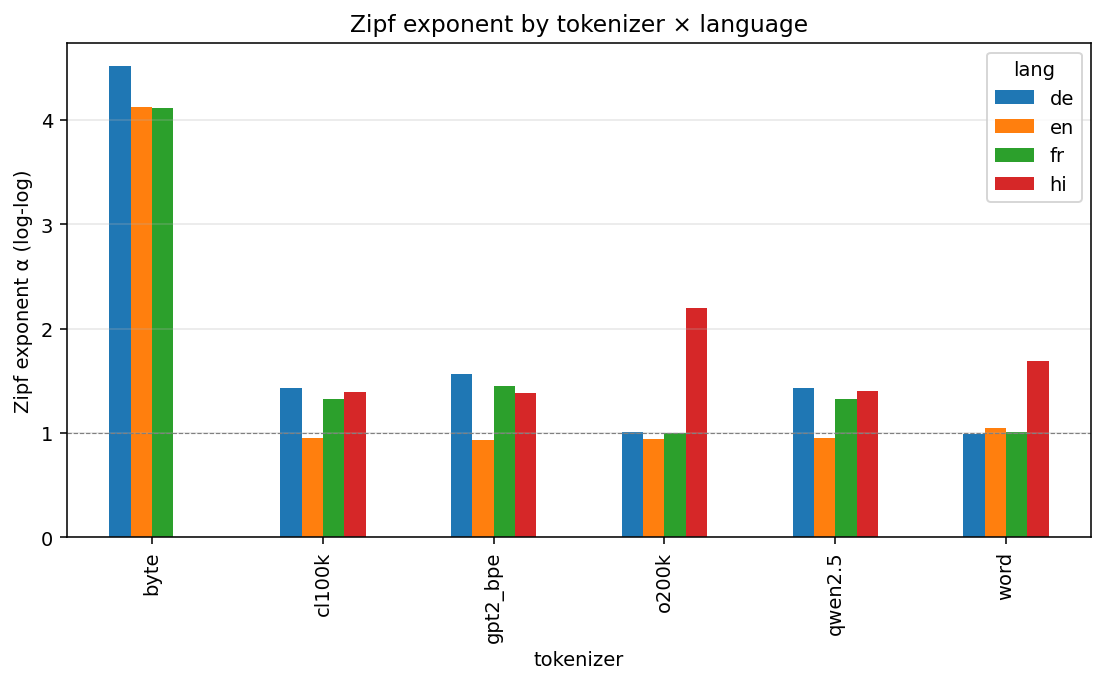
\includegraphics[width=0.85\linewidth]{../plots/alpha_cross_lang.png}
  \caption{Per-(tokenizer, language) $\alpha$ for the original three-language run plus Hindi.
    Turkish was subsequently included per the same protocol to improve typological coverage
    (agglutinative baseline); the same pre-registered GRADUATE/KILL decision rule was applied
    identically, and its results appear in Table~\ref{tab:crosslang}. The Hindi word baseline
    ($\approx 1.7$) is anomalously high, which is why Hindi $\Delta\alpha$ is treated as a
    boundary case rather than a main result.}
  \label{fig:crosslang}
\end{figure}

\section{Code and Reproducibility}
\label{app:code}

All scripts are available in the \texttt{tokenizer-zipf/} directory of the supplementary
material:

\begin{itemize}
  \item \texttt{scripts/01\_pull\_corpus.py}: streams Wikipedia via HuggingFace Datasets
    and saves plain-text article samples per language.
  \item \texttt{scripts/02\_tokenize.py}: applies each tokenizer and pickles
    \texttt{collections.Counter} objects.
  \item \texttt{scripts/03\_fit\_zipf.py}: fits power laws (log-log OLS and CSN MLE),
    writes \texttt{notes/alpha\_table.csv}.
  \item \texttt{scripts/04\_plot\_zipf.py}: generates all figures in \texttt{plots/}.
  \item \texttt{scripts/05\_synthetic\_mechanism.py}: corpus-free fragmentation simulation (Table~\ref{tab:synth}).
  \item \texttt{scripts/06\_fit\_mandelbrot.py}: Zipf--Mandelbrot fits with a fitting-window sweep.
  \item \texttt{scripts/07\_add\_languages.py}: Turkish and Chinese pull/tokenize/fit.
  \item \texttt{scripts/08\_critique\_analysis.py}: fertility-vs-regime correlations, bootstrap CIs, $x_{\min}$ sensitivity.
  \item \texttt{scripts/09\_downstream.py}: bits-per-byte of Qwen2.5-1.5B per language (original four).
  \item \texttt{scripts/10\_expand\_downstream.py}: expands downstream to seven languages (adds Spanish, Italian, Finnish; Table~\ref{tab:down}).
  \item \texttt{run.sh}: sequential runner with timestamped logging.
\end{itemize}

\textbf{Environment.} Python 3.10, \texttt{tiktoken 0.13.0}, \texttt{powerlaw 2.0.0},
\texttt{transformers 4.x}, \texttt{numpy}, \texttt{scipy}, \texttt{pandas},
\texttt{matplotlib}. All packages are user-installable via \texttt{pip}.

\textbf{Compute.} All experiments ran on a single CPU core. Total wall time $\approx 90$
minutes (dominated by Wikipedia streaming and tokenization).

\section{Pre-registered Decision Rule}
\label{app:prereg}

Prior to running any experiments, the following decision rule was documented in
\texttt{tokenizer-zipf/hypotheses.md}:

\begin{quote}
  \textbf{GRADUATE} if $\geq 3$ of the 6 tokenizers show $|\Delta\alpha| > 0.05$ vs.\
  word-level baseline, \emph{and} power-law fits have KS distance $< 0.05$.

  \textbf{KILL} if all tokenizers give $\alpha$ within $\pm 0.03$ of word-level (no shift)
  \emph{or} if KS distance $> 0.10$ across all tokenizers.
\end{quote}

Outcome: all four subword tokenizers met $|\Delta\alpha| > 0.05$ (range: 0.102--0.121) with
KS $< 0.02$ for English; the pre-registered GRADUATE rule was met decisively.

%%%%%%%%%%%%%%%%%%%%%%%%%%%%%%%%%%%%%%%%%%%%%%%%%%%%%%%%%%%%

\newpage

\section*{Conference For AI Scientists 2026 - AI Involvement Checklist}
\label{checklist_ai_involvement}

\subsection*{Research Stage Assessment}

\begin{enumerate}

  \item \textbf{Hypothesis development}

    Answer: \involvementD{}

    Iteration Effort: \iterationMedium{}

    Explanation: The hypothesis that BPE tokenizers distort Zipf statistics was proposed
    by a frontier large language model. The human researcher gave high-level direction
    (requesting novel 2-hour research investigations in any domain) and approved three
    candidate hypotheses from a pool of 20 generated by the AI. The AI performed
    literature survey, novelty assessment, and pre-registration of the decision rule.
    Approximately 20--30 iterations were spent generating and refining the idea pool
    before the final hypothesis was selected.

  \item \textbf{Experimental design and implementation}

    Answer: \involvementD{}

    Iteration Effort: \iterationMedium{}

    Explanation: The AI system designed the full experiment: corpus selection, tokenizer
    set, fitting procedures, pre-registered decision rule, and output formats. All five
    analysis scripts were written by the AI. The human had no involvement in coding or
    experimental setup beyond approving the plan at a high level. Approximately 10--20
    substantive iterations were needed to handle data-pull failures (Wikipedia rate
    limits, HuggingFace streaming issues) and a pivot from Mistral-7B to Qwen2.5.

  \item \textbf{Analysis of data and interpretation of results}

    Answer: \involvementD{}

    Iteration Effort: \iterationLow{}

    Explanation: Analysis was run end-to-end by the AI. The cross-language pattern
    (direction reversal for German/French, o200k exception) was identified and
    interpreted by the AI without human guidance. The human reviewed the final numerical
    results summary.

  \item \textbf{Writing}

    Answer: \involvementD{}

    Iteration Effort: \iterationLow{}

    Explanation: This paper was written by a frontier large language model following the
    CAISc 2026 template. The human author reviewed the paper before submission.
    Approximately 1--3 drafting passes were made.

\end{enumerate}

\subsection*{AI System Documentation}

\begin{enumerate}
  \setcounter{enumi}{4}

  \item \textbf{AI systems used}

    Description: A frontier large language model with extended context and tool-use
    capabilities served as the primary researcher. The system had access to a Python
    execution environment, web search, and file system tools. All data collection,
    analysis, and writing was performed by this system within a single multi-hour
    interactive session.

  \item \textbf{Observed AI Limitations}

    Description: The AI system exhibited several failure modes. (1)~It initially
    proposed specific numerical constants (e.g., for Mandelbrot's correction parameter)
    without empirical basis, which were caught in a self-critique pass. (2)~The system
    initially over-counted the number of tokenizers meeting the decision rule (reporting
    ``5/5'' when the correct count was 4 subword tokenizers), a subtle categorization
    error. (3)~The system's literature awareness is limited to its training cutoff and
    may miss very recent publications on tokenizer statistics. (4)~In a second analysis
    round, the system initially over-framed $\Delta\alpha$ as a novel diagnostic; an
    adversarial self-critique found it correlates with the existing fertility metric at
    $r = 0.92$ and predicts downstream cost no better than fertility, prompting the more
    conservative two-regime \emph{shape}-characterisation framing adopted here. The
    cross-language mechanism, left informal in the first version, is now derived under an
    idealised fragmentation model (Appendix~\ref{app:deriv}), though real BPE departs from
    that idealisation.

\end{enumerate}

\newpage

\section*{Conference For AI Scientists 2026 - Reproducibility and Responsibility Checklist}
\label{checklist_reproducibility}

\begin{enumerate}

\item {\bf Claims}
    \item[] Question: Do the main claims made in the abstract and introduction accurately reflect the paper's contributions and scope?
    \item[] Answer: \answerYes{}
    \item[] Justification: The two-regime characterisation (mid-range flattening with bootstrap CIs; tail steepening), the fertility relationship ($r = 0.92$ across four languages including Turkish), the synthetic crossover, the tail-vs-fertility orthogonality ($r = -0.93$), and the downstream bits-per-byte correlation ($r = 0.90$, $n=7$) are each supported by the corresponding tables (Tables~\ref{tab:english}--\ref{tab:down}, \ref{tab:synth}) and Appendix~\ref{app:deriv}. We explicitly state where fertility is the simpler predictor, so the abstract does not overclaim a novel diagnostic. The pre-registered decision rule and outcome are documented in Appendix~\ref{app:prereg}.

\item {\bf Limitations}
    \item[] Question: Does the paper discuss the limitations of the work performed by the authors?
    \item[] Answer: \answerYes{}
    \item[] Justification: Section~\ref{sec:limitations} discusses corpus size, fitting method bias, and limited language coverage. Appendix~\ref{app:deriv} provides a formal derivation of the fragmentation crossover under an idealized model; a derivation covering the full BPE merge process with co-occurrence structure remains future work.

\item {\bf Theory assumptions and proofs}
    \item[] Question: For each theoretical result, does the paper provide the full set of assumptions and a complete (and correct) proof?
    \item[] Answer: \answerNA{}
    \item[] Justification: This is an empirical paper with no theoretical results; no proofs are required.

\item {\bf Experimental result reproducibility}
    \item[] Question: Does the paper fully disclose all the information needed to reproduce the main experimental results?
    \item[] Answer: \answerYes{}
    \item[] Justification: Data sources, tokenizers (with package versions), corpus sizes, and fitting procedures are described in Section~\ref{sec:methods}. Full code is described in Appendix~\ref{app:code} and provided in supplementary material.

\item {\bf Open access to data and code}
    \item[] Question: Does the paper provide open access to the data and code?
    \item[] Answer: \answerYes{}
    \item[] Justification: The Wikipedia corpus is publicly available via HuggingFace Datasets (\url{https://huggingface.co/datasets/wikimedia/wikipedia}). All tokenizer packages are open source. Analysis code is provided in the supplementary material.

\item {\bf Experimental setting/details}
    \item[] Question: Does the paper specify all the training and test details necessary to understand the results?
    \item[] Answer: \answerYes{}
    \item[] Justification: Section~\ref{sec:methods} specifies corpus version, article count, token counts, tokenizer vocabulary sizes, fitting range (ranks 10--10,000), and the KS diagnostic. Package versions are given in Appendix~\ref{app:code}.

\item {\bf Experiment statistical significance}
    \item[] Question: Does the paper report error bars or other appropriate information about statistical significance?
    \item[] Answer: \answerYes{}
    \item[] Justification: We report token-level multinomial bootstrap 95\% confidence intervals on every $\alpha_{\text{loglog}}$ ($B = 500$; e.g., word/en $1.051\,[1.050,1.051]$, cl100k/en $0.947\,[0.946,0.947]$), and all subword-vs-word CIs are disjoint, so the mid-range $\Delta\alpha$ shifts are significant. We additionally report the Pearson correlation ($r = 0.92$, 95\% CI $[0.87, 0.97]$) between fertility and mid-range $\Delta\alpha$, and KS distances for the CSN fits (Appendix~\ref{app:csn}).

\item {\bf Experiments compute resources}
    \item[] Question: Does the paper provide sufficient information on compute resources?
    \item[] Answer: \answerYes{}
    \item[] Justification: Appendix~\ref{app:code} states that all experiments ran on a single CPU core with approximately 90 minutes total wall time.

\item {\bf Research Ethics}
    \item[] Question: Does the research conform with the NeurIPS Code of Ethics?
    \item[] Answer: \answerYes{}
    \item[] Justification: This paper analyzes publicly available text (Wikipedia) and open-source software. No human subjects, sensitive data, or harmful applications are involved. AI authorship is disclosed per CAISc policies.

\item {\bf Broader impacts}
    \item[] Question: Does the paper discuss both potential positive and negative societal impacts?
    \item[] Answer: \answerYes{}
    \item[] Justification: The Discussion section notes that the Zipfian fingerprint may benefit low-resource NLP practitioners (positive) and that it reveals systematic distortions in LLM training data statistics (neutral/informational). No harmful applications are identified; this is a measurement and characterization paper.

\end{enumerate}

\end{document}
